\documentclass[10pt]{extarticle}

%SOME USEFUL PACKAGES
\usepackage[portuguese]{babel}
\usepackage{extsizes}
\usepackage[reqno]{amsmath} % equation numbers on the right
\usepackage{amsmath}
\usepackage{amssymb}
\usepackage{amsthm}
\usepackage{amscd}
\usepackage{amsfonts}
\usepackage{graphicx}
\usepackage{dsfont}
\usepackage{fancyhdr}
\usepackage{enumerate}
\usepackage[utf8]{inputenc}
\usepackage{booktabs}
\usepackage{listings}
\usepackage[margin=1in]{geometry}
\usepackage[hypcap]{caption}
\usepackage{longtable}
\usepackage{etoolbox}
%\usepackage[alf]{abntex2cite}
\usepackage[siunitx]{circuitikz}
\usepackage{tikz}
\usepackage{enumitem}
\usepackage{algpseudocode}
\usepackage{algorithm}


\usepackage{verbatim}
\usepackage{float}
\usepackage{indentfirst}

%HEADER
\pagestyle{fancy}\lhead{Vinícius Julião Ramos} \rhead{DCC207 - Algoritmos II - 2020.1}
\chead{{\large{\bf }}} \lfoot{} \rfoot{\bf \thepage} 
\cfoot{}


\title{ \textsc{Universidade Federal de Minas Gerais} \\ \textsc{Departamento de Ciência da Computação} \\ \bigskip TP1 -- Árvore de Sufixos}

\author{Vinícius Julião Ramos \\ \normalsize{viniciusjuliao@dcc.ufmg.br}}

\date{\today}

\begin{document}
\maketitle

\begin{abstract}
O trabalho aqui apresentado consiste na elaboração de um modelo computacional
que consiga resolver o problema de encontrar a maior \textit{substring} que
se repete em um texto.
Para isso solicitou-se que fosse realizada a construção de uma árvore de sufixos
e a partir dessa arvore, se encontrasse a cadeia de caracteres com o maior
tamanho e que se repete.
\end{abstract}
    
\section{Introdução}
\section{Introdução}

Para possibilitar a virtualização de um roteador, através de um aplicação,
necessitou-se utilizar um protocolo da camada de transporte.
Nesse cenário, optou-se pelo UDP, uma vez que esse protocolo é o que mais se
aproxima da camada de rede, pelo motivo de não fornecer quaisquer garantias
de entrega, controle de erros ou gerenciamento de conexão.
Portanto, para esse socket, uma classe \textbf{Router} foi criada com a
finalidade de gerenciar a troca de informações.
Essa mesma classe é responsável por executar comandos em duas \textit{thread}
diferentes, sendo que uma delas recebe comandos da entrada padrão do sistema e 
a outra executa o protocolo de rede especificado pelo trabalho.

A opção de criar uma classe separada para gerenciar a tabela de roteamento
permitiu gerênciar todas a funções que cabem à uma tabela de roteamento: a
remoção de rotas desatualizadas, a montagem da lista de distâncias através
do \textit{Split Horizon} e também o rerroteamente imediato. Essa última função
é desempenhada por demanda, o que permite que a melhor rota para determinado
endereço seja calculada apenas quando o roteador envia mensagem para tal
destino. Já a atualização periódica de rotas é uma atividade conjunta entre o
roteador e a tabela de roteamento; a tabela de roteamento entrega ao roteador
a lista de distâncias, mas cabe ao roteador atualizar os vizinhos de acordo com
o período especificado.
\newpage

\section{Modelagem}
% falar da modelagem

Assim como citado na sessão anterior, a árvore de sufixos foi criada com base
numa \textit{trie compacta}.
Isso significa que o objetivo dessa estrutura é tentar minimizar o custo de
espaço.
Para isso, cada nó, ao invés de armazenar \textit{sub strings} provenientes
do texto original, armazena uma tupla com um valor \texttt{inicio} e
\texttt{fim}.
Essa tupla representa os índices de determinada substring contida no texto
fazendo com que a rearmazenagem do texto não seja necessária e redundante,
por consequência.
Além disso, é valido ressaltar que o grafo foi implementado através de uma lista
de adjacências.
Sendo assim, as arestas da árvore são representadas por uma lista contendo todos
os nós filhos de um nó pai, não existindo uma estrutura de dados criada
especificamente para descrever as aresta, uma vez que trata-se apenas de um
link entre dois nós, nessa implementação.
Conclui-se portanto, que todas as informações são armazenadas nos nós.

Um outro fator que mere relevância é a adição de um atributo \textit{booleano}
na estrutura \textbf{nó}.
O objetivo dessa informação é apenas indicar se determinado nó da árvore pode
ser identificado como um um sufixo do texto.
Em algumas notações de implementação, costuma-se utilizar o caractere cifrão
('\$') para tal representação.
Porém, apenas por uma questão de generalização, optou-se por não adicionar um
caractere especial ao texto a fim de garantir que tal solução funcione mesmo
para os casos em que esse símbolo faça parte do alfabeto do texto.
Dessa maneira, a estrutura do tipo \textbf{Nó} é denotada por:

\begin{figure}[h]
	\begin{center}
		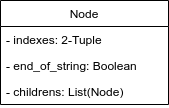
\includegraphics[scale=0.75]{Figuras/node.png}
	\end{center}
	\caption{\label{fig:node} Estrutura de um nó.}
\end{figure}

A partir do modelo de nó da Figura \ref{fig:node} a árvore de sufixos é
construída.
A classe que controla árvore tem apenas dois atributos, um deles é do tipo
\textbf{Nó} e representa a raíz da árvore.
Já o outro atributo é o texto o qual a árvore será montada.
Portanto os nós internos da árvore são obtidos apenas no caminhamento recursivo
entre os nós que estão "abaixo" da raiz.
Em resumo, com excessão da raíz da árvore, nenhum dos demais nós é um atributo
próprio da classe \textbf{SufixTree}.
Isso faz com que o princípio do encapsulamento seja garantido.

\begin{figure}[h]
	\begin{center}
		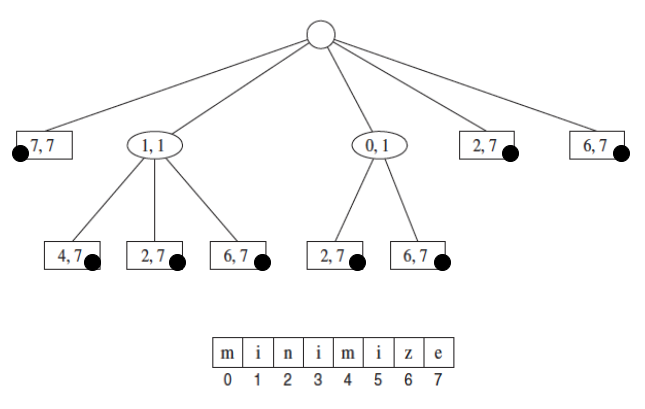
\includegraphics[scale=0.5]{Figuras/compact-trie.png}
	\end{center}
    \caption{\label{fig:compact-trie} Exemplo de uma árvore de sufixos para a palavra "minimize".}
\end{figure}


A Figura \ref{fig:compact-trie} representa como se daria uma árvore a partir da
solução empregada nesse trabalho.
Relacionando as Figuras \ref{fig:node} e \ref{fig:compact-trie} temos que o par
de número inteiros contidos no interior de cada nó se trata do atributo
\texttt{indexes}, o circulo preto indica que a marcação de fim de string é
verdadeiro.
Porém, a lista de adjacência é expressada para cada aresta que parte de um nó em
direção a um nó mais profundo.
Pode-se tomar como exemplo o nó \texttt{(0, 1)} que tem \texttt{(2, 7)} e
\texttt{(6, 7)} em sua lista de adjacências.

% \newpage

\section{Decisões de implementação}
Como a solução desse problema consiste em duas etapas que são executada
separadamente, essa seção detalhará cada uma das etapas e suas respectivas
peculiaridades.

\subsection{Construção da árvore} 
Esse é o passo fundamental do problema, uma vez que para realizar qualquer
operação na árvore de sufixos, é necessário antes de tudo criar a
estrutura.
O algoritmo de montagem da árvore foi inspirado na explicação de um vídeo
\footnote{https://www.youtube.com/watch?v=VA9m\_l6LpwI}
e tem como ponto chave o algoritmo de busca de um a trie.
Dado um sufixo $s_i$ do texto, o algoritmo tenta realizar \textit{matchs}
parciais, entre algum prefixo de $s_i$ e o texto representado pelos nós
da árvore.
Ocorrendo um encontro parcial entre $s_i$ e um nó $N$, $s_i$ é atualizada, retirando
o prefixo que fora compatível com $N$, então reinicia-se a busca entre os
filhos de $N$ recursivamente.
Quando a busca se depara com uma substring $s_i$ (atualizada) que não
houve um \textit{match} parcial, então um novo nó é criado para tal substring.
Nesse cenário, o último nó o qual houve um encontro parcial de caracteres se
torna o nó "pai" do novo nó.
Em resumo o algoritmo de busca e construção consiste em consumir prefixos de
$s_i$, que é atualizado a cada etapa que o prefixos é encontrado no nó,
e então sufixo restante que não fora compatível é adicionado como um nó folha.
O nó inicial da busca é a raiz da árvore, e assume-se por nulidade que na raiz
já ocorre um match parcial.

Há um \textit{border case} na inserção que merece atenção:
Quando ocorre um \textit{match} parcial tanto para uma substring $ss$ de $s_i$
quanto para o nó $t$, ou seja, a substring $ss_t$ contida no nó não é uma
substring de $s_i$, então o $t$ deverá ser dividido em dois nós (um pai $t_p$ e
um filho $t_f$).
Nesse caso, a divisão será de tal forma que:
\begin{itemize}
    \item $t_p$ conterá o match parcial entre $t$ e $s_i$, $t_f$ conterá o
    \item $t_f$ conterá o restante de $t$ que não deu match com $s_i$, sendo que
    toda a sub árvore com a raiz em $t$, agora terá $t_f$ como raiz.
    \item um novo nó $h$ será criado a partir do resto de $s_i$ que não combinou
    com a substring em $t$. O nó $h$ será um nó folha, filho de $t_p$.
\end{itemize}

Por fim, pode-se afirmar que a montagem da árvore de sufixos tem um comportamento
assintótico em $O(n^2)$.
Essa afirmação é trivial, uma vez que é sabido que o custo da busca de uma
substring de tamanho $m$ em uma árvore de sufixos é $O(m)$.
Para inserir os $n$ sufixos do texto $Q$ em uma árvore de sufixos, deve-se
realizar $n$ buscas de tamanho $1, 2, 3, .... n-2, n-1, n$ -- uma para cada
sufixo, e então encontrar a posição que o novo nó será criado.
Assim, o custo dessa inserção é a soma de uma progressão aritmética e tem como
fórmula: 

$$\sum_{i=1}^{n}i = \frac{n(n-1)}{2} = O(\frac{n^2-n}{2}) = O(n^2)$$


\subsection{Encontrar a maior substring que se repete}
Nesse algoritmo, há a necessidade de uma execução recursiva, em que uma chamada
mais distante do topo da pilha de recursão deverá aplicar uma função
\textit{max} para as chamadas internas.
Para isso, o algoritmo escolhido foi uma busca em profundidade, em que o nó
pai da árvore deverá obter o \textit{max} dentre os nós filhos, mas com algumas
exceções.
A seguinte expressão recursiva demonstrará a execução da computação do DFS:

\[ biggest\_substr(t) = 
    \begin{cases}
        (repetitions = 0, size = 0) \quad \text{if t is a leaf node} \\
        \\
        (repetitions = \text{quantity(t.childrens)}, size = \text{t.size}) \\
        \quad \quad \quad \text{if all t.childrens are leaf nodes}\\
        \\
        (repetitions, size) = max(\text{for each biggest\_subtr(t.childrens)}) \\
         \quad \quad \quad \text{if one of t.childrens is not a leaf}
    \end{cases}
\]

Vale expressar que a função $max$, para cada retorno de $biggest\_substr()$,
realiza uma comparação entre a melhor substring atual e a obtida com o
retorno da função, então se o retorno for uma melhor escolha que o atual,
uma troca acontece.
Essa validação ocorre de forma a obter o melhor conjunto
$(repetitions, size)$ o qual é o par que tem maior valor $size$ e que
$repetitions > 1$, ou seja, a maior substring que acontece mais de uma vez.
Observe que a partir do momento em que $biggest\_substr()$ é chamada passando
a raiz da árvore como parâmetro, se a raiz não possui nós folha e nem é uma folha
por si só, então o terceiro caso será executado, chamando $biggest\_substr()$
para todos os filhos da raiz.
Esse fato acontece sucessivamente até que se chegue ao primeiro caso base (em
que o nó é uma folha) e se retorne para o segundo (no qual todos os filhos do
nó são folhas).

Pode-se dizer então que a função $max$ é executada quando o "desempilhamento"
das chamadas recursivas acontece, ou seja, é necessário que a busca em
profundidade que parte de $t$ retorne até $t$ para que o estado $t.(repetitions,
size)$ seja computado.
Assim, quando $t$ terminar as chamadas de $biggest\_substring()$ para todos os
filhos, obterá a melhor escolha.
De posse da melhor escolha $c = (rep, siz)$, a chamada que solicitou
$biggest\_substring()$ para $t$ deverá retornar o par $(c.rep, c.siz + t.size)$,
pois o tamanho de $t$ deve ser incrementado à melhor escolha.
A quantidade de repetições não mudará na computação de $biggest\_substring(t)$,
pois as repetições são computadas em função da quantidade de nós folha que a
sub árvore com raiz em $t$ possui.

A função de encontrar a maior string que se repete no texto é a codificação
das afirmações feitas acima.
Entretanto, para possibilitar a obtenção dos índices da string desejada, o
retorno da função não se trata de $(repetitions, size)$ mas sim $(repetitions,
indexes)$.
Nesse caso, $indexes$ se refere aos índices de inicio e fim da maior substring
que se repete e a partir desses índices é possível obter o tamanho apenas com
uma subtração.

Para determinar o comportamento assintótico da busca da maior substring que se
repete, serão tomadas duas afirmações como base.
Levando em consideração que a árvore fora escrita a partir de um texto $T$ de
tamanho $n$, ou seja, $T$ possui $n$ sufixos diferentes.
Dito isto, pode-se afirmar que:
\begin{enumerate}
    \item A quantidade de nós folha da árvore de sufixo é igual $n$.
    É possível verificar tal afirmação, validando que a construção da árvore
    consiste na criação de nós folha para cada sufixo de $T$.
    Uma vez que a busca da posição correta para adicionar um novo sufixo $s_i$
    parte do princípio de consumir o maior prefixo possível de $s_i$,
    o que restará após tal busca é um sufixo restante de $s_i$ (que também é um
    sufixo de $T$) e que se tornará uma nova folha.
    \item A quantidade de nós intermediários na árvore é no máximo igual a $n-1$.
    Pela criação da árvore, nunca haverá um nó intermediário que possua apenas um
    nó filho, pois a criação de nós intermediários parte do caso de borda citado
    na subseção anterior.
    Ou seja, um nó intermediário é criado apenas em \textit{splits}.
    Assim, para um nível $j$ da árvore com $m$ nós a quantidade máxima de nós
    no nível $j-1$ é igual a $m \div 2$, sendo o caso em que cada nó de $j-1$
    tem apenas dois filhos.
    Por fim, visto o caso da máxima existência de nós pai (2 filhos por nó),
    para a árvore completa de $n$ folhas com $l$ níveis, pode-se obter a
    quantidade de nós intermediários pela soma: $\sum_{i=0}^{l-1}2^i = 2^l-1 = n-1$,
    pois o $i$-ésimo nível de uma árvore binária completa, possui $2^{i-1}$ nós.
\end{enumerate}

Tomando as duas afirmações como base, e o algoritmo de busca em profundidade,
pode-se afirmar que $n$ nós folha serão visitados e no máximo $n-1$ nós
intermediários.
Isso significa que, uma vez que a visita a cada nó tem custo $O(1)$ o custo total
da busca de maior substring é $O(2n-1) = O(n)$.

\subsection{Custo de espaço}

As duas afirmações da subseção anterior, permitem admitir que no máximo $2n-1$
nó são criados.
Então, por hora, ignorando as arestas do grafo, o custo de memória $O(n)$.
Porém, como uma árvore é um grafo direcional acíclico, em que um nó não possui
mais de um nó "pai", a quantidade de arestas é igual a quantidade de nós na árvore
decrescido de $1$, pois o nó raiz não possui predecessor.
Logo a quantidade de arestas é no máximo $2n-2$.
Portanto o custo de memória do grafo é uma soma de $2n-1$ nós mais $2n-2$ arestas,
o que resulta em $O(n)$ para o custo de espaço.

% \newpage

\section{Análise Experimental}
Nesse ponto, serão apresentados dados da execução da solução apresentada pelo
trabalho.
Algumas imagens serão demonstradas demonstrando o tempo de execução e a memória
utilizada.
Vale ressaltar que os tempos de execução foram computados usando o temporizador
nativo do Python pela biblioteca texttt{time} sendo que o tempo da leitura do
arquivo de entrada foi ignorado.
A obtenção da memória utilizada pelo programa foram obtidos pelo uso do Valgrind.
Além disso as funções que imprimem a saída também foram removidas nas análises.
O comando para executar a solução do trabalho usando o arquivo
\texttt{sarscov2.fasta} é:

\lstset{language=bash}
\begin{lstlisting}[frame=single]
$ python3 main.py sarscov2.fasta
\end{lstlisting}

\begin{figure}[h]
	\begin{center}
		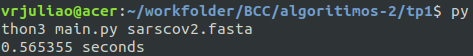
\includegraphics[scale=0.75]{Figuras/create-trie.png}
	\end{center}
	\caption{\label{fig:create-trie} Tempo de criação da árvore (processamento dos sufixos).}
\end{figure}

Na Figura \ref{fig:create-trie} apenas a linha que computa
\texttt{tree = sufix\_tree.SufixTree(text)} é considerada.
Da mesma forma computou-e o tempo de execução da obtenção da maior substring
que se repete na árvore apenas pelo tempo da chamada
\texttt(repetitions, indexes = tree.biggest\_substr()), e o tempo é obsevado
na Figura \ref{fig:biggest-substr}.

\begin{figure}[h]
	\begin{center}
		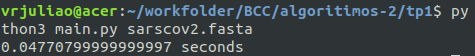
\includegraphics[scale=0.75]{Figuras/biggest-substr.png}
	\end{center}
	\caption{\label{fig:biggest-substr} Tempo para encontrar a maior substring que se repete na árvore.}
\end{figure}

Já o tempo total de execução foi obtido através considerando toda a função
\texttt{main}, incluindo o tempo de leitura da entrada e a impressão da resposta.
Dessa forma, a Figura \ref{fig:total-execution} demonstra a resposta que a
solução dá para o arquivo \texttt{sarscov2.fasta}.
A primeira linha representa a quantidade de repetições encontradas, a próxima
linha mostra a substring que se repete.
Por fim, a ultima linha impressa é referente ao tempo de execução de toda a
função principal.

\begin{figure}[h]
	\begin{center}
		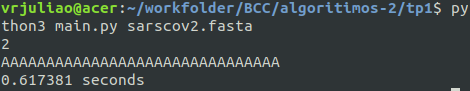
\includegraphics[scale=0.75]{Figuras/total-execution.png}
	\end{center}
	\caption{\label{fig:total-execution} Tempo total de execução.}
\end{figure}


A resposta obtida pelo Valgrind é demonstrada na Figura \ref{fig:valgrind}, que
demonstra uma alocação total de $7.936.935$ bytes.
O comando executado para a obtenção dessa resposta foi:
\lstset{language=bash}
\begin{lstlisting}[frame=single]
$ valgrind --tool=memcheck python3 -E -tt main.py sarscov2.fasta
\end{lstlisting}

\begin{figure}[h]
	\begin{center}
		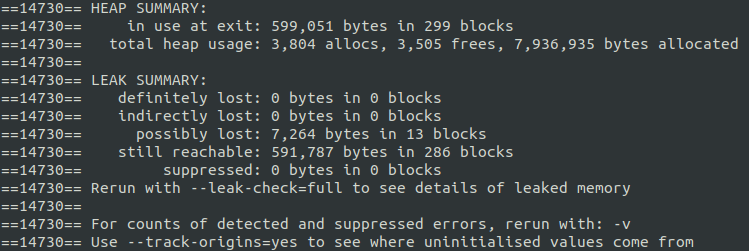
\includegraphics[scale=0.5]{Figuras/valgrind.png}
	\end{center}
	\caption{\label{fig:valgrind} Execução do Valgrind para obtenção da memória utilizada.}
\end{figure}

\section{Conclusão}
Através da análise assintótica das duas funções e da observação das respostas
de tempo de execução da solução para a entrada passada, pôde-se concluir
que há uma grande diferença entre os tempos de obtenção da maior string e 
do processamento de sufixos.
Entretanto pode-se realizar um experimento com diversas entradas (de tamanhos
variados) para observar os tempos de execução de cada uma das funções e então
traçar um gráfico.
Nesse experimento, o comportamento do gráfico que computa os sufixos, terá uma
curva que remete à uma função polinômial quadrática.
Já a obtenção da maior substring que se repete o comportamento do gráfico é um
polinômio de grau 1.

A elaboração desse trabalho mostrou quão rápido é a manipulação de textos utilizando
uma árvore de sufixos compacta.
Apesar do custo elevado de construção da árvore apresentado nesse trabalho, existem
alternativas de construção da árvore com um custo menor que $O(n^2)$.
Esse fato torna a árvore de sufixos extremamente útil e aplicável em manipulações de
textos.

% \begin{thebibliography}{9}

% \bibitem{cplusplus}
%     http://www.cplusplus.com 27 nov. 2019
    
% \bibitem{book:DFS}
%     Jon Kleinberg, Eva Tardos. 2006. \textit{Algorithm Design} (1st Edition, p 83). Pearson - Addison Wesley.
    
% \bibitem{book:BFS}
%     Jon Kleinberg, Eva Tardos. 2006. \textit{Algorithm Design} (1st Edition, p 79). Pearson - Addison Wesley.

% \bibitem{book:DAG}
%     Jon Kleinberg, Eva Tardos. 2006. \textit{Algorithm Design} (1st Edition, p 99 - 101). Pearson - Addison Wesley.
    
% \bibitem{cpp:vector}
%     http://www.cplusplus.com/reference/vector/vector 27 nov. 2019
    
% \bibitem{cpp:stack}
%     http://www.cplusplus.com/reference/stack/stack 27 nov. 2019
    
% \bibitem{cpp:iostream}
%     http://www.cplusplus.com/reference/iostream 27 nov. 2019
    
% \bibitem{cpp:chronos}
%     http://www.cplusplus.com/reference/chrono 27 nov. 2019
% \end{thebibliography}
\end{document}